% Root file used ashow macros
\documentclass{beamer}
\usepackage{tikz}
\usetikzlibrary{calc}
\usepackage{xcolor}
\usepackage{multicol}
\usepackage{amsmath}
\usepackage{amssymb}

% ================================================================
% Answer-overlay helpers
% ================================================================
\newcommand{\ablank}[1]{%
  \alt<2>{\textcolor{red}{#1}}{\underline{\phantom{#1}}}%
}
\newcommand{\ashow}[1]{\uncover<2->{\textcolor{red}{\small #1}}}
\newcommand{\ashowq}[1]{\alt<2->{\textcolor{red}{\small #1}}{?}}

% Answers drawn straight on to a TikZ diagram, revealed on overlay 2 like \ashow.
% Space is reserved on overlay 1, so the diagram does not move between slides.
\usetikzlibrary{overlay-beamer-styles}
\tikzset{
  ans/.style     = {red, thick, visible on=<2->},
  ansfill/.style = {red!15, visible on=<2->},
  anslab/.style  = {red, font=\tiny, visible on=<2->},
}

\title{Fractions: Adding \& Subtracting}
\author{}
\date{}

\begin{document}

\frame{\titlepage}

\begin{frame}{Contents}
\small
\begin{columns}[T]
\column{0.5\textwidth}
\textbf{Questions and short answers}
\begin{itemize}
  \item \hyperlink{q-st1}{\beamergotobutton{Starter 1}}
  \item \hyperlink{q-st2}{\beamergotobutton{Starter 2}}
  \item \hyperlink{q-st3}{\beamergotobutton{Starter 3}}
  \item \hyperlink{q-st4}{\beamergotobutton{Starter 4}}
  \item \hyperlink{q-st5}{\beamergotobutton{Starter 5}}
\end{itemize}
\column{0.5\textwidth}
\textbf{Worked solutions}
\begin{itemize}
  \item \hyperlink{work-st1}{\beamergotobutton{Starter 1}}
  \item \hyperlink{work-st2}{\beamergotobutton{Starter 2}}
  \item \hyperlink{work-st3}{\beamergotobutton{Starter 3}}
  \item \hyperlink{work-st4}{\beamergotobutton{Starter 4}}
  \item \hyperlink{work-st5}{\beamergotobutton{Starter 5}}
\end{itemize}
\end{columns}
\end{frame}

% ================================================================
% Starter 1
% ================================================================
\begin{frame}{Starter 1}
\hypertarget{q-st1}{}

\vspace{-2em}

\begin{columns}

\column{0.2\textwidth}
\begin{center}
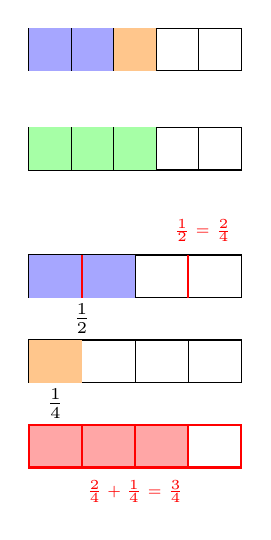
\begin{tikzpicture}[scale=0.9]

\draw (0,1) rectangle (3,1.6);
\fill[blue!35] (0,1) rectangle (1.2,1.6);
\fill[orange!45] (1.2,1) rectangle (1.8,1.6);
\foreach \x in {0.6,1.2,1.8,2.4} \draw (\x,1) -- (\x,1.6);
\draw (0,-0.4) rectangle (3,0.2);
\fill[green!35] (0,-0.4) rectangle (1.8,0.2);
\foreach \x in {0.6,1.2,1.8,2.4} \draw (\x,-0.4) -- (\x,0.2);

\draw (0,-2.2) rectangle (3,-1.6);
\draw (1.5,-2.2) -- (1.5,-1.6);
\fill[blue!35] (0,-2.2) rectangle (1.5,-1.6);
\node at (0.75,-2.5) {\small $\frac{1}{2}$};
\draw (0,-3.4) rectangle (3,-2.8);
\foreach \x in {0.75,1.5,2.25} \draw (\x,-3.4) -- (\x,-2.8);
\fill[orange!45] (0,-3.4) rectangle (0.75,-2.8);
\node at (0.375,-3.7) {\small $\frac{1}{4}$};

% --- Q6 answer: split the half into quarters, then 2/4 + 1/4 = 3/4 ---
\draw[ans] (0.75,-2.2) -- (0.75,-1.6);
\draw[ans] (2.25,-2.2) -- (2.25,-1.6);
\node[anslab, above left] at (3,-1.55) {$\tfrac{1}{2}=\tfrac{2}{4}$};
\fill[ansfill, red!35] (0,-4.6) rectangle (2.25,-4.0);
\draw[ans] (0,-4.6) rectangle (3,-4.0);
\foreach \x in {0.75,1.5,2.25} \draw[ans] (\x,-4.6) -- (\x,-4.0);
\node[anslab, below] at (1.5,-4.65) {$\tfrac{2}{4}+\tfrac{1}{4}=\tfrac{3}{4}$};
\end{tikzpicture}
\end{center}

\column{0.8\textwidth}
\small
\begin{enumerate}
  \item Fully simplify: $\dfrac{12}{16}$ \ashow{$=\frac{3}{4}$}
  \item Which is larger: $\dfrac{3}{7}$ or $\dfrac{3}{9}$? \ashow{$\frac{3}{7}$}
  \item Convert $\dfrac{11}{4}$ to a mixed number. \ashow{$=2\frac{3}{4}$}
  \item Complete the addition represented by the bars to the left: $$\color{blue}\dfrac{\text{{\ashowq{2}}}}{5} \color{orange} + \dfrac{\text{{\ashowq{1}}}}{5} \color{green} = \dfrac{3}{\text{{\ashowq{5}}}}$$
  \item Calculate:
  \[
    \frac{1}{7} + \frac{3}{7} \qquad \frac{5}{9} + \frac{2}{9}
  \]
  \ashow{$=\frac{4}{7},\ \frac{7}{9}$}
  \item To add $\dfrac{1}{2} + \dfrac{1}{4}$, what must you do first? Can you draw a picture to demonstrate? \ashow{Find a common denominator: $\frac12=\frac24$, so $\frac24+\frac14=\frac34$.}

\begin{multicols}{2}
  \item Calculate: $\dfrac{1}{2} + \dfrac{1}{4}$ \ashow{$=\frac{3}{4}$}
  \item Calculate: $\dfrac{1}{3} + \dfrac{1}{4}$ \ashow{$=\frac{7}{12}$}
\end{multicols}
\end{enumerate}

\end{columns}
\end{frame}

\begin{frame}{Worked Solution: Starter 1, Question 1}
\hypertarget{work-st1}{}
\textbf{Question:} Fully simplify $\dfrac{12}{16}$.

\textbf{Worked Solution:} \ashow{Divide the numerator and denominator by their HCF, $4$: $\frac{12}{16}=\frac{12\div4}{16\div4}=\frac34$.}
\end{frame}

\begin{frame}{Worked Solution: Starter 1, Question 2}
\textbf{Question:} Which is larger: $\dfrac{3}{7}$ or $\dfrac{3}{9}$?

\textbf{Worked Solution:} \ashow{Same numerator, smaller denominator gives the larger fraction: $\frac37>\frac39$, so $\frac37$ is larger.}
\end{frame}

\begin{frame}{Worked Solution: Starter 1, Question 3}
\textbf{Question:} Convert $\dfrac{11}{4}$ to a mixed number.

\textbf{Worked Solution:} \ashow{Since $11\div4=2$ remainder $3$, $\frac{11}{4}=2\frac34$.}
\end{frame}

\begin{frame}{Worked Solution: Starter 1, Question 4}
\textbf{Question:} Complete the addition represented by the bars to the left:
\[
\color{blue}\dfrac{\text{{\ashowq{2}}}}{5} \color{orange} + \dfrac{\text{{\ashowq{1}}}}{5} \color{green} = \dfrac{3}{\text{{\ashowq{5}}}}
\]

\textbf{Worked Solution:} \ashow{The first bar shows $2$ blue fifths and $1$ orange fifth, which together make $3$ green fifths: $\frac25+\frac15=\frac35$.}
\end{frame}

\begin{frame}{Worked Solution: Starter 1, Question 5}
\textbf{Question:} Calculate:
\[
\frac{1}{7} + \frac{3}{7} \qquad \frac{5}{9} + \frac{2}{9}
\]

\textbf{Worked Solution:} \ashow{Add the numerators and keep the denominator the same: $\frac{1+3}{7}=\frac47$ and $\frac{5+2}{9}=\frac79$.}
\end{frame}

\begin{frame}{Worked Solution: Starter 1, Question 6}
\textbf{Question:} To add $\dfrac{1}{2}+\dfrac{1}{4}$, what must you do first? Can you draw a picture to demonstrate?

\textbf{Worked Solution:} \ashow{First rewrite $\frac12$ with denominator $4$: $\frac12=\frac24$. Then $\frac24+\frac14=\frac34$. A picture can show the half split into two quarters, so two quarters plus one quarter is three quarters.}
\end{frame}

\begin{frame}{Worked Solution: Starter 1, Question 7}
\textbf{Question:} Calculate: $\dfrac{1}{2}+\dfrac{1}{4}$.

\textbf{Worked Solution:} \ashow{$\frac12+\frac14=\frac24+\frac14=\frac34$.}
\end{frame}

\begin{frame}{Worked Solution: Starter 1, Question 8}
\textbf{Question:} Calculate: $\dfrac{1}{3}+\dfrac{1}{4}$.

\textbf{Worked Solution:} \ashow{Use a common denominator of $12$: $\frac13+\frac14=\frac{4}{12}+\frac{3}{12}=\frac{7}{12}$.}
\end{frame}

% ================================================================
% Starter 2
% ================================================================
\begin{frame}{Starter 2}
\hypertarget{q-st2}{}

\vspace{-2em}

\begin{columns}

\column{0.2\textwidth}

\begin{center}

\vspace{-5em}
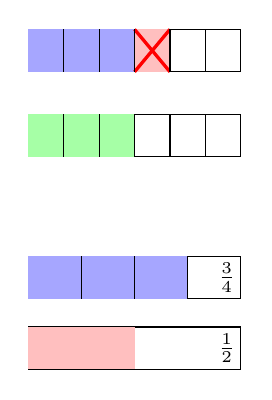
\begin{tikzpicture}[scale=0.9]

\draw (0,4) rectangle (3,4.6);
\fill[blue!35] (0,4) rectangle (2,4.6);
\fill[red!25] (1.5,4) rectangle (2,4.6);
\draw[red, very thick] (1.5,4) -- (2,4.6);
\draw[red, very thick] (2,4) -- (1.5,4.6);
\foreach \x in {0.5,1,1.5,2,2.5} \draw (\x,4) -- (\x,4.6);

\draw (0,2.8) rectangle (3,3.4);
\fill[green!35] (0,2.8) rectangle (1.5,3.4);
\foreach \x in {0.5,1,1.5,2,2.5} \draw (\x,2.8) -- (\x,3.4);

\draw (0,0.8) rectangle (3,1.4);
\fill[blue!35] (0,0.8) rectangle (2.25,1.4);
\foreach \x in {0.75,1.5,2.25} \draw (\x,0.8) -- (\x,1.4);
\node at (2.8,1.1) {\small $\frac{3}{4}$};

\draw (0,-0.2) rectangle (3,0.4);
\draw (1.5,-0.2) -- (1.5,0.4);
\fill[red!25] (0,-0.2) rectangle (1.5,0.4);
\node at (2.8,0.1) {\small $\frac{1}{2}$};

\end{tikzpicture}
\end{center}

\column{0.8\textwidth}
\small
\begin{enumerate}
  \item Write 3 fractions equivalent to $\dfrac{2}{3}$. \ashow{$\frac46,\frac69,\frac{8}{12}$}
  \item Order smallest to largest: $\dfrac{1}{8}, \ \dfrac{1}{2}, \ \dfrac{1}{12}$ \ashow{$\frac{1}{12}<\frac{1}{8}<\frac{1}{2}$}
  \item Convert $2\dfrac{3}{7}$ to an improper fraction. \ashow{$=\frac{17}{7}$}
  \item Complete the subtraction represented by the bars to the left: $$\color{blue}\dfrac{4}{6} \color{red}- \dfrac{\text{{\ashowq{1}}}}{6} \color{green} = \dfrac{\text{{\ashowq{3}}}}{6} \color{black} = \dfrac{1}{\text{{\ashowq{2}}}}$$
  \item Calculate:
  \[
    \frac{7}{10} - \frac{3}{10} \qquad \frac{8}{9} - \frac{5}{9}
  \]
  \ashow{$=\frac{2}{5},\ \frac{1}{3}$}
  \item Use the bars to work out $\dfrac{3}{4} - \dfrac{1}{2}$. \ashow{$=\frac{1}{4}$}
  \begin{multicols}{2}
  \item Calculate: $\dfrac{5}{6} - \dfrac{1}{4}$ \ashow{$=\frac{7}{12}$}
  \item Calculate: $\dfrac{7}{8} - \dfrac{2}{3}$ \ashow{$=\frac{5}{24}$}
  \end{multicols}
  \vspace{-2em}
  \item Order smallest to largest: $\dfrac{3}{8},\ \dfrac{1}{2},\ \dfrac{5}{12}$ \ashow{$\frac{3}{8}<\frac{5}{12}<\frac{1}{2}$}
\end{enumerate}

\end{columns}
\end{frame}

\begin{frame}{Worked Solution: Starter 2, Question 1}
\hypertarget{work-st2}{}
\textbf{Question:} Write $3$ fractions equivalent to $\dfrac{2}{3}$.

\textbf{Worked Solution:} \ashow{Multiply the numerator and denominator by the same number: $\frac23=\frac46=\frac69=\frac{8}{12}$.}
\end{frame}

\begin{frame}{Worked Solution: Starter 2, Question 2}
\textbf{Question:} Order smallest to largest: $\dfrac{1}{8},\ \dfrac{1}{2},\ \dfrac{1}{12}$.

\textbf{Worked Solution:} \ashow{Use denominator $24$: $\frac18=\frac{3}{24}$, $\frac12=\frac{12}{24}$, $\frac{1}{12}=\frac{2}{24}$, so $\frac{1}{12}<\frac{1}{8}<\frac{1}{2}$.}
\end{frame}

\begin{frame}{Worked Solution: Starter 2, Question 3}
\textbf{Question:} Convert $2\dfrac{3}{7}$ to an improper fraction.

\textbf{Worked Solution:} \ashow{$2\frac37=\frac{2\times7+3}{7}=\frac{17}{7}$.}
\end{frame}

\begin{frame}{Worked Solution: Starter 2, Question 4}
\textbf{Question:} Complete the subtraction represented by the bars to the left:
\[
\color{blue}\dfrac{4}{6} \color{red}- \dfrac{\text{{\ashowq{1}}}}{6} \color{green} = \dfrac{\text{{\ashowq{3}}}}{6} \color{black} = \dfrac{1}{\text{{\ashowq{2}}}}
\]

\textbf{Worked Solution:} \ashow{Starting from $\frac46$, remove one sixth; the green bar shows $\frac36$ left, which simplifies to $\frac12$.}
\end{frame}

\begin{frame}{Worked Solution: Starter 2, Question 5}
\textbf{Question:} Calculate:
\[
\frac{7}{10} - \frac{3}{10} \qquad \frac{8}{9} - \frac{5}{9}
\]

\textbf{Worked Solution:} \ashow{Subtract the numerators and keep the denominator: $\frac{7-3}{10}=\frac{4}{10}=\frac25$ and $\frac{8-5}{9}=\frac39=\frac13$.}
\end{frame}

\begin{frame}{Worked Solution: Starter 2, Question 6}
\textbf{Question:} Use the bars to work out $\dfrac{3}{4}-\dfrac{1}{2}$.

\textbf{Worked Solution:} \ashow{Rewrite $\frac12$ as $\frac24$; the bars show $\frac34$ take away the shaded half leaves one quarter: $\frac34-\frac24=\frac14$.}
\end{frame}

\begin{frame}{Worked Solution: Starter 2, Question 7}
\textbf{Question:} Calculate: $\dfrac{5}{6}-\dfrac{1}{4}$.

\textbf{Worked Solution:} \ashow{Use denominator $12$: $\frac56-\frac14=\frac{10}{12}-\frac{3}{12}=\frac{7}{12}$.}
\end{frame}

\begin{frame}{Worked Solution: Starter 2, Question 8}
\textbf{Question:} Calculate: $\dfrac{7}{8}-\dfrac{2}{3}$.

\textbf{Worked Solution:} \ashow{Use denominator $24$: $\frac78-\frac23=\frac{21}{24}-\frac{16}{24}=\frac{5}{24}$.}
\end{frame}

\begin{frame}{Worked Solution: Starter 2, Question 9}
\textbf{Question:} Order smallest to largest: $\dfrac{3}{8},\ \dfrac{1}{2},\ \dfrac{5}{12}$.

\textbf{Worked Solution:} \ashow{Use denominator $24$: $\frac38=\frac{9}{24}$, $\frac12=\frac{12}{24}$, $\frac{5}{12}=\frac{10}{24}$, so $\frac38<\frac{5}{12}<\frac12$.}
\end{frame}

% ================================================================
% Starter 3
% ================================================================
\begin{frame}{Starter 3}
\hypertarget{q-st3}{}

\vspace{-2em}

\begin{columns}

\column{0.3\textwidth}
\vspace{-5em}
\begin{center}
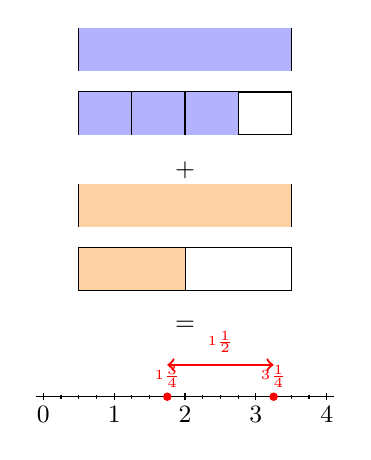
\begin{tikzpicture}[scale=0.9]
% Two wholes side by side as bars (1 3/4 + 1 1/2)
% 1st whole
\draw (0,5) rectangle (3,5.6);
\fill[blue!30] (0,5) rectangle (3,5.6);
% 3/4 part
\draw (0,4.1) rectangle (3,4.7);
\fill[blue!30] (0,4.1) rectangle (2.25,4.7);
\foreach \x in {0.75,1.5,2.25} \draw (\x,4.1) -- (\x,4.7);
\node at (1.5,3.6) {\small $+$};
% 2nd whole
\draw (0,2.8) rectangle (3,3.4);
\fill[orange!35] (0,2.8) rectangle (3,3.4);
% 1/2 part
\draw (0,1.9) rectangle (3,2.5);
\draw (1.5,1.9) -- (1.5,2.5);
\fill[orange!35] (0,1.9) rectangle (1.5,2.5);
\node at (1.5,1.4) {\small $=$};
% Number line
\draw (-0.6,0.4) -- (3.6,0.4);
\foreach \x/\lab in {0/0,1/1,2/2,3/3,4/4} {
  \draw (\x-0.5,0.35) -- (\x-0.5,0.45);
  \node at (\x-0.5,0.15) {\small \lab};
}
\foreach \x in {0,1,2,3} {
  \foreach \q in {0.25,0.5,0.75} {
    \draw (\x+\q-0.5,0.37) -- (\x+\q-0.5,0.43);
  }
}

% --- Q5 answer: the two mixed numbers marked, with the difference between them ---
\fill[ans] (1.25,0.4) circle (0.06);
\node[anslab, above, inner sep=2pt] at (1.25,0.45) {$1\tfrac{3}{4}$};
\fill[ans] (2.75,0.4) circle (0.06);
\node[anslab, above, inner sep=2pt] at (2.75,0.45) {$3\tfrac{1}{4}$};
\draw[ans, <->] (1.25,0.85) -- (2.75,0.85);
\node[anslab, above] at (2,0.88) {$1\tfrac{1}{2}$};
\end{tikzpicture}
\end{center}

\column{0.7\textwidth}
\small
\begin{enumerate}
\begin{multicols}{3}
  \item $\dfrac{2}{5} + \dfrac{1}{5}$ \ashow{$=\frac{3}{5}$}
  \item $\dfrac{3}{4} - \dfrac{1}{2}$ \ashow{$=\frac{1}{4}$}
  \item Simplify: $\dfrac{36}{48}$ \ashow{$=\frac{3}{4}$}
\end{multicols}
  
  \item Fill in the blanks using the diagram:
  \[
    \color{blue}\text{{\ashowq{1}}}\frac{\text{{\ashowq{3}}}}{4} \color{orange} + 1\frac{\text{{\ashowq{1}}}}{\text{{\ashowq{2}}}} \color{black} = \frac{\text{{\ashowq{7}}}}{4} + \frac{\text{{\ashowq{6}}}}{4} = \frac{\text{{\ashowq{13}}}}{4} = \ \text{{\ashowq{3}}}  \frac{1}{\text{{\ashowq{4}}}}
  \]
  \begin{multicols}{2}
  \item 
  \[
    2\frac{1}{3} + 1\frac{1}{3}
  \]
  \ashow{$=3\frac{2}{3}$}
  \item 
  \[
    3\frac{1}{4} + 1\frac{1}{2}
  \]
  \ashow{$=4\frac{3}{4}$}
  \end{multicols}
  \item Mark $1\dfrac{3}{4}$ and $3\dfrac{1}{4}$ on the number line. What is the difference? How else could you work this out? \ashow{Difference $=\frac{3}{2}=1\frac12$; work out as $3\frac14-1\frac34=\frac{13}{4}-\frac{7}{4}=\frac{6}{4}=\frac{3}{2}$.}
  \begin{multicols}{2}
  \item Calculate: $2\dfrac{2}{3} + 1\dfrac{3}{4}$ \ashow{$=4\frac{5}{12}$}
  \item Calculate $1\dfrac{3}{4} - 3\dfrac{1}{4} $ \ashow{$=-1\frac{1}{2}$}
  \end{multicols}
\end{enumerate}

\end{columns}
\end{frame}

\begin{frame}{Worked Solution: Starter 3, Question 1}
\hypertarget{work-st3}{}
\textbf{Question:} $\dfrac{2}{5}+\dfrac{1}{5}$.

\textbf{Worked Solution:} \ashow{$\frac25+\frac15=\frac{2+1}{5}=\frac35$.}
\end{frame}

\begin{frame}{Worked Solution: Starter 3, Question 2}
\textbf{Question:} $\dfrac{3}{4}-\dfrac{1}{2}$.

\textbf{Worked Solution:} \ashow{Rewrite $\frac12$ as $\frac24$: $\frac34-\frac24=\frac14$.}
\end{frame}

\begin{frame}{Worked Solution: Starter 3, Question 3}
\textbf{Question:} Simplify: $\dfrac{36}{48}$.

\textbf{Worked Solution:} \ashow{HCF of $36$ and $48$ is $12$: $\frac{36}{48}=\frac{36\div12}{48\div12}=\frac34$.}
\end{frame}

\begin{frame}{Worked Solution: Starter 3, Question 4}
\textbf{Question:} Fill in the blanks using the diagram:
\[
\color{blue}\text{{\ashowq{1}}}\frac{\text{{\ashowq{3}}}}{4} \color{orange} + 1\frac{\text{{\ashowq{1}}}}{\text{{\ashowq{2}}}} \color{black} = \frac{\text{{\ashowq{7}}}}{4} + \frac{\text{{\ashowq{6}}}}{4} = \frac{\text{{\ashowq{13}}}}{4} = \ \text{{\ashowq{3}}} \frac{1}{\text{{\ashowq{4}}}}
\]

\textbf{Worked Solution:} \ashow{The diagram shows $1\frac34=\frac74$ and $1\frac12=\frac64$, so $\frac74+\frac64=\frac{13}{4}=3\frac14$.}
\end{frame}

\begin{frame}{Worked Solution: Starter 3, Question 5}
\textbf{Question:}
\[
2\frac{1}{3}+1\frac{1}{3}
\]

\textbf{Worked Solution:} \ashow{$2\frac13+1\frac13 = \frac73+\frac43=\frac{11}{3}=3\frac23$.}
\end{frame}

\begin{frame}{Worked Solution: Starter 3, Question 6}
\textbf{Question:}
\[
3\frac{1}{4}+1\frac{1}{2}
\]

\textbf{Worked Solution:} \ashow{$3\frac14+1\frac12 = \frac{13}{4}+\frac64=\frac{19}{4}=4\frac34$.}
\end{frame}

\begin{frame}{Worked Solution: Starter 3, Question 7}
\textbf{Question:} Mark $1\dfrac{3}{4}$ and $3\dfrac{1}{4}$ on the number line. What is the difference? How else could you work this out?

\textbf{Worked Solution:} \ashow{The difference is $3\frac14-1\frac34=\frac{13}{4}-\frac74=\frac64=\frac32=1\frac12$. Alternatively, count the number of quarters from $1\frac34$ to $3\frac14$; there are $6$ quarters, i.e.\ $1\frac12$.}
\end{frame}

\begin{frame}{Worked Solution: Starter 3, Question 8}
\textbf{Question:} Calculate: $2\dfrac{2}{3}+1\dfrac{3}{4}$.

\textbf{Worked Solution:} \ashow{$\frac83+\frac74 = \frac{32}{12}+\frac{21}{12}=\frac{53}{12}=4\frac{5}{12}$.}
\end{frame}

\begin{frame}{Worked Solution: Starter 3, Question 9}
\textbf{Question:} Calculate $1\dfrac{3}{4}-3\dfrac{1}{4}$.

\textbf{Worked Solution:} \ashow{$\frac74-\frac{13}{4}=-\frac64=-\frac32=-1\frac12$.}
\end{frame}

% ================================================================
% Starter 4
% ================================================================
\begin{frame}{Starter 4}
\hypertarget{q-st4}{}

\vspace{-2em}
\begin{columns}
\column{0.25\textwidth}

\vspace{-7em}

\begin{center}
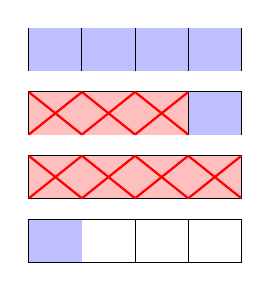
\begin{tikzpicture}[scale=0.9]
% Show 13/4 as bars (3 whole bars + 1/4)
\foreach \y in {3.8,2.9,2.0} {
  \draw (0,\y) rectangle (3,\y+0.6);
  \fill[blue!25] (0,\y) rectangle (3,\y+0.6);
  \foreach \x in {0.75,1.5,2.25} \draw (\x,\y) -- (\x,\y+0.6);
}
\draw (0,1.1) rectangle (3,1.7);
\foreach \x in {0.75,1.5,2.25} \draw (\x,1.1) -- (\x,1.7);
\fill[blue!25] (0,1.1) rectangle (0.75,1.7);

% Cross out 1 3/4 = 7 quarter-segments
% That's all 4 quarters of one whole bar + 3 quarters of another
% Cross out all 4 quarters of the bottom whole bar (y=2.0)
\foreach \i in {0,1,2,3} {
  \fill[red!25] ({0.75*\i},2.0) rectangle ({0.75*\i+0.75},2.6);
  \draw[red, thick] ({0.75*\i},2.0) -- ({0.75*\i+0.75},2.6);
  \draw[red, thick] ({0.75*\i+0.75},2.0) -- ({0.75*\i},2.6);
}
% Cross out 3 quarters of the next bar (y=2.9)
\foreach \i in {0,1,2} {
  \fill[red!25] ({0.75*\i},2.9) rectangle ({0.75*\i+0.75},3.5);
  \draw[red, thick] ({0.75*\i},2.9) -- ({0.75*\i+0.75},3.5);
  \draw[red, thick] ({0.75*\i+0.75},2.9) -- ({0.75*\i},3.5);
}

\end{tikzpicture}
\end{center}

\column{0.75\textwidth}
\small
\begin{enumerate}
  
  \item Which is greater: $2\dfrac{1}{3}$ or $2\dfrac{2}{5}$? \ashow{$2\frac{2}{5}$}
  \item Convert $\dfrac{23}{6}$ to a mixed number. \ashow{$=3\frac{5}{6}$}
  \item Consider the diagram on the left, fill in the blanks to demonstrate subtraction using improper fractions:
  \[
    3\frac{1}{4} - 1\frac{3}{4} = \frac{\text{{\ashowq{13}}}}{4} - \frac{\text{{\ashowq{7}}}}{4} = \frac{\text{{\ashowq{6}}}}{4} = \ \text{{\ashowq{1}}} \frac{\text{{\ashowq{2}}}}{\text{{\ashowq{4}}}}
  \]
  \begin{multicols}{2}
  \item
  \[
    3\frac{3}{5} - 1\frac{1}{5}
  \]
  \ashow{$=2\frac{2}{5}$}
  \item 
  \[
   4\frac{5}{6} - 2\frac{1}{6}
  \]
  \ashow{$=2\frac{2}{3}$}
  \end{multicols}
  \begin{multicols}{2}
  \item \[ 1\dfrac{2}{3} + 2\dfrac{1}{4} \] \ashow{$=3\frac{11}{12}$}
  \item
  \[
    4\frac{1}{4} - 1\frac{1}{2}  
  \]
  \ashow{$=2\frac{3}{4}$}
  \end{multicols}
\begin{multicols}{2}
  \item 
  \[
    3\frac{1}{3} - 1\frac{3}{4}
  \]
  \ashow{$=1\frac{7}{12}$}

  \item \[ 5\dfrac{1}{3} - 2\dfrac{3}{4} \] \ashow{$=2\frac{7}{12}$}
\end{multicols}
  
\end{enumerate}

\end{columns}
\end{frame}

\begin{frame}{Worked Solution: Starter 4, Question 1}
\hypertarget{work-st4}{}
\textbf{Question:} Which is greater: $2\dfrac{1}{3}$ or $2\dfrac{2}{5}$?

\textbf{Worked Solution:} \ashow{Compare the fractional parts: $\frac13=\frac{5}{15}$ and $\frac25=\frac{6}{15}$, so $2\frac13<2\frac25$; hence $2\frac25$ is greater.}
\end{frame}

\begin{frame}{Worked Solution: Starter 4, Question 2}
\textbf{Question:} Convert $\dfrac{23}{6}$ to a mixed number.

\textbf{Worked Solution:} \ashow{$23\div6=3$ remainder $5$, so $\frac{23}{6}=3\frac56$.}
\end{frame}

\begin{frame}{Worked Solution: Starter 4, Question 3}
\textbf{Question:} Consider the diagram on the left, fill in the blanks to demonstrate subtraction using improper fractions:
\[
3\frac{1}{4} - 1\frac{3}{4} = \frac{\text{{\ashowq{13}}}}{4} - \frac{\text{{\ashowq{7}}}}{4} = \frac{\text{{\ashowq{6}}}}{4} = \ \text{{\ashowq{1}}} \frac{\text{{\ashowq{2}}}}{\text{{\ashowq{4}}}}
\]

\textbf{Worked Solution:} \ashow{Convert: $3\frac14=\frac{13}{4}$ and $1\frac34=\frac74$; then $\frac{13}{4}-\frac74=\frac64=1\frac24=1\frac12$.}
\end{frame}

\begin{frame}{Worked Solution: Starter 4, Question 4}
\textbf{Question:}
\[
3\frac{3}{5} - 1\frac{1}{5}
\]

\textbf{Worked Solution:} \ashow{$3\frac35-1\frac15 = \frac{18}{5}-\frac65=\frac{12}{5}=2\frac25$.}
\end{frame}

\begin{frame}{Worked Solution: Starter 4, Question 5}
\textbf{Question:}
\[
4\frac{5}{6} - 2\frac{1}{6}
\]

\textbf{Worked Solution:} \ashow{$4\frac56-2\frac16 = \frac{29}{6}-\frac{13}{6}=\frac{16}{6}=\frac83=2\frac23$.}
\end{frame}

\begin{frame}{Worked Solution: Starter 4, Question 6}
\textbf{Question:}
\[
1\frac{2}{3} + 2\frac{1}{4}
\]

\textbf{Worked Solution:} \ashow{$\frac53+\frac94 = \frac{20}{12}+\frac{27}{12}=\frac{47}{12}=3\frac{11}{12}$.}
\end{frame}

\begin{frame}{Worked Solution: Starter 4, Question 7}
\textbf{Question:}
\[
4\frac{1}{4} - 1\frac{1}{2}
\]

\textbf{Worked Solution:} \ashow{$4\frac14-1\frac12 = \frac{17}{4}-\frac64=\frac{11}{4}=2\frac34$.}
\end{frame}

\begin{frame}{Worked Solution: Starter 4, Question 8}
\textbf{Question:}
\[
3\frac{1}{3} - 1\frac{3}{4}
\]

\textbf{Worked Solution:} \ashow{$\frac{10}{3}-\frac74 = \frac{40}{12}-\frac{21}{12}=\frac{19}{12}=1\frac{7}{12}$.}
\end{frame}

\begin{frame}{Worked Solution: Starter 4, Question 9}
\textbf{Question:}
\[
5\frac{1}{3} - 2\frac{3}{4}
\]

\textbf{Worked Solution:} \ashow{$\frac{16}{3}-\frac{11}{4} = \frac{64}{12}-\frac{33}{12}=\frac{31}{12}=2\frac{7}{12}$.}
\end{frame}

% ================================================================
% Starter 5
% ================================================================
\begin{frame}{Starter 5}
\hypertarget{q-st5}{}

\vspace{-2em}

\begin{columns}

\column{0.2\textwidth}
\begin{center}
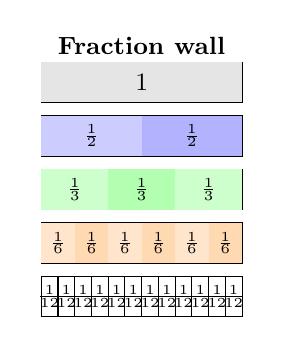
\begin{tikzpicture}[scale=0.85]

\node at (1.5,0.85) {\small\textbf{Fraction wall}};

\draw (0,0) rectangle (3,0.6);
\fill[gray!20] (0,0) rectangle (3,0.6);
\node at (1.5,0.3) {\small $1$};

\draw (0,-0.8) rectangle (3,-0.2);
\draw (1.5,-0.8) -- (1.5,-0.2);
\fill[blue!20] (0,-0.8) rectangle (1.5,-0.2);
\fill[blue!30] (1.5,-0.8) rectangle (3,-0.2);
\node at (0.75,-0.5) {\tiny $\frac{1}{2}$};
\node at (2.25,-0.5) {\tiny $\frac{1}{2}$};

\draw (0,-1.6) rectangle (3,-1.0);
\foreach \x in {1,2} \draw (\x,-1.6) -- (\x,-1.0);
\fill[green!20] (0,-1.6) rectangle (1,-1.0);
\fill[green!30] (1,-1.6) rectangle (2,-1.0);
\fill[green!20] (2,-1.6) rectangle (3,-1.0);
\node at (0.5,-1.3) {\tiny $\frac{1}{3}$};
\node at (1.5,-1.3) {\tiny $\frac{1}{3}$};
\node at (2.5,-1.3) {\tiny $\frac{1}{3}$};

\draw (0,-2.4) rectangle (3,-1.8);
\foreach \x in {0.5,1,1.5,2,2.5} \draw (\x,-2.4) -- (\x,-1.8);
\foreach \i/\col in {0/orange!20,1/orange!30,2/orange!20,3/orange!30,4/orange!20,5/orange!30} {
  \fill[\col] ({0.5*\i},-2.4) rectangle ({0.5*\i+0.5},-1.8);
  \node at ({0.5*\i+0.25},-2.1) {\tiny $\frac{1}{6}$};
}

\draw (0,-3.2) rectangle (3,-2.6);
\foreach \x in {0.25,0.5,...,2.75} \draw (\x,-3.2) -- (\x,-2.6);
\foreach \i in {0,...,11} {
  \node at ({0.25*\i+0.125},-2.9) {\tiny $\frac{1}{12}$};
}

\end{tikzpicture}
\end{center}

\column{0.8\textwidth}
\small
\begin{enumerate}
\begin{multicols}{2}
\item Fully simplify: $\dfrac{15}{20}$ \ashow{$=\frac{3}{4}$}
\item Fully simplify: $\dfrac{72}{96}$ \ashow{$=\frac{3}{4}$}
\end{multicols}
  \item Use the fraction wall to fill in the blanks:
  \[
    \frac{1}{2} + \frac{\text{{\ashowq{3}}}}{6} = 1 \qquad \frac{\text{{\ashowq{1}}}}{3} + \frac{\text{{\ashowq{4}}}}{6} = 1
  \] 
\begin{multicols}{2}
  \item $2\dfrac{3}{4} + 1\dfrac{2}{3}$ \ashow{$=4\frac{5}{12}$}
  \item $4\dfrac{1}{5} - 1\dfrac{3}{4}$ \ashow{$=2\frac{9}{20}$}
\end{multicols}  
  \item Maya says: \textit{``$\frac{1}{2} + \frac{1}{3} = \frac{2}{5}$''}. Explain the mistake and find the correct answer. \ashow{She added the denominators too; use a common denominator: $\frac36+\frac26=\frac56$.}
  \item Amir eats $\dfrac{3}{8}$, Beth eats $\dfrac{1}{4}$, Cal eats $\dfrac{1}{3}$ of a pizza. What fraction is left? \ashow{$\frac{1}{24}$}
  \item Fill in the blanks: $\quad 3\dfrac{1}{4} + \ablank{1\frac{11}{12}} = 5\dfrac{1}{6}$
  \item True or false? $\dfrac{a}{b} + \dfrac{a}{c} = \dfrac{2a}{b+c}$. Can you explain your answer with a proof/counterexample? \ashow{False; e.g.\ $a=b=c=1$ gives $2=1$. Correct: $\frac ab+\frac ac=\frac{a(c+b)}{bc}$.}
\end{enumerate}

\end{columns}
\end{frame}

\begin{frame}{Worked Solution: Starter 5, Question 1}
\hypertarget{work-st5}{}
\textbf{Question:} Fully simplify: $\dfrac{15}{20}$.

\textbf{Worked Solution:} \ashow{HCF of $15$ and $20$ is $5$: $\frac{15}{20}=\frac{15\div5}{20\div5}=\frac34$.}
\end{frame}

\begin{frame}{Worked Solution: Starter 5, Question 2}
\textbf{Question:} Fully simplify: $\dfrac{72}{96}$.

\textbf{Worked Solution:} \ashow{HCF of $72$ and $96$ is $24$: $\frac{72}{96}=\frac{72\div24}{96\div24}=\frac34$.}
\end{frame}

\begin{frame}{Worked Solution: Starter 5, Question 3}
\textbf{Question:} Use the fraction wall to fill in the blanks:
\[
\frac{1}{2} + \frac{\text{{\ashowq{3}}}}{6} = 1 \qquad \frac{\text{{\ashowq{1}}}}{3} + \frac{\text{{\ashowq{4}}}}{6} = 1
\]

\textbf{Worked Solution:} \ashow{Using the wall, $\frac12=\frac36$, so $\frac12+\frac36=1$; and $\frac13=\frac26$, so $\frac26+\frac46=1$, which is the same as $\frac13+\frac46=1$.}
\end{frame}

\begin{frame}{Worked Solution: Starter 5, Question 4}
\textbf{Question:} $2\dfrac{3}{4}+1\dfrac{2}{3}$.

\textbf{Worked Solution:} \ashow{$\frac{11}{4}+\frac53 = \frac{33}{12}+\frac{20}{12}=\frac{53}{12}=4\frac{5}{12}$.}
\end{frame}

\begin{frame}{Worked Solution: Starter 5, Question 5}
\textbf{Question:} $4\dfrac{1}{5}-1\dfrac{3}{4}$.

\textbf{Worked Solution:} \ashow{$\frac{21}{5}-\frac74 = \frac{84}{20}-\frac{35}{20}=\frac{49}{20}=2\frac{9}{20}$.}
\end{frame}

\begin{frame}{Worked Solution: Starter 5, Question 6}
\textbf{Question:} Maya says: \textit{``$\frac{1}{2}+\frac{1}{3}=\frac{2}{5}$''}. Explain the mistake and find the correct answer.

\textbf{Worked Solution:} \ashow{She added the denominators as well as the numerators. Use a common denominator: $\frac12+\frac13=\frac36+\frac26=\frac56$.}
\end{frame}

\begin{frame}{Worked Solution: Starter 5, Question 7}
\textbf{Question:} Amir eats $\dfrac{3}{8}$, Beth eats $\dfrac{1}{4}$, Cal eats $\dfrac{1}{3}$ of a pizza. What fraction is left?

\textbf{Worked Solution:} \ashow{Total eaten: $\frac38+\frac14+\frac13 = \frac{9}{24}+\frac{6}{24}+\frac{8}{24}=\frac{23}{24}$. Left: $1-\frac{23}{24}=\frac{1}{24}$.}
\end{frame}

\begin{frame}{Worked Solution: Starter 5, Question 8}
\textbf{Question:} Fill in the blanks: $\quad 3\dfrac{1}{4} + \ablank{1\frac{11}{12}} = 5\dfrac{1}{6}$.

\textbf{Worked Solution:} \ashow{Subtract $3\frac14$ from $5\frac16$: $5\frac16-3\frac14 = \frac{31}{6}-\frac{13}{4} = \frac{62}{12}-\frac{39}{12}=\frac{23}{12}=1\frac{11}{12}$.}
\end{frame}

\begin{frame}{Worked Solution: Starter 5, Question 9}
\textbf{Question:} True or false? $\dfrac{a}{b}+\dfrac{a}{c}=\dfrac{2a}{b+c}$. Can you explain your answer with a proof/counterexample?

\textbf{Worked Solution:} \ashow{False. Take $a=b=c=1$: the left side is $1+1=2$, but the right side is $\frac{2}{2}=1$. In fact $\frac ab+\frac ac=\frac{a(c+b)}{bc}$.}
\end{frame}

\end{document}